\section{Applications}
\label{wmtk:sec:applications}

To showcase the generality and effectiveness of our approach, we implement five popular mesh editing algorithms in our framework, and compare them with reference implementations. Overall, the performance of our method are competitive for surface applications, but the overhead due to the approach generality is higher in 3D, leading to higher running time.

\paragraph{Shortest Edge Collapsing}

The simplest algorithm for simplifying a triangle edge is shortest edge collapse \cite{hoppe1996progressive}, which performs a series of collapse operations prioritizing the shorter edges. The algorithm requires only one local operation, edge collapse. A common criteria for termination is reaching a desired number of mesh elements. We compare our implementation with the ``decimate'' implementation in libigl \cite{jacobson2016libigl}. The serial libigl implementation is comparable when running the algorithms serially, and our parallel implementation is up to 9 times faster when using 32 threads (Figure \ref{fig:decimate}).

\begin{figure}
    \centering\footnotesize
    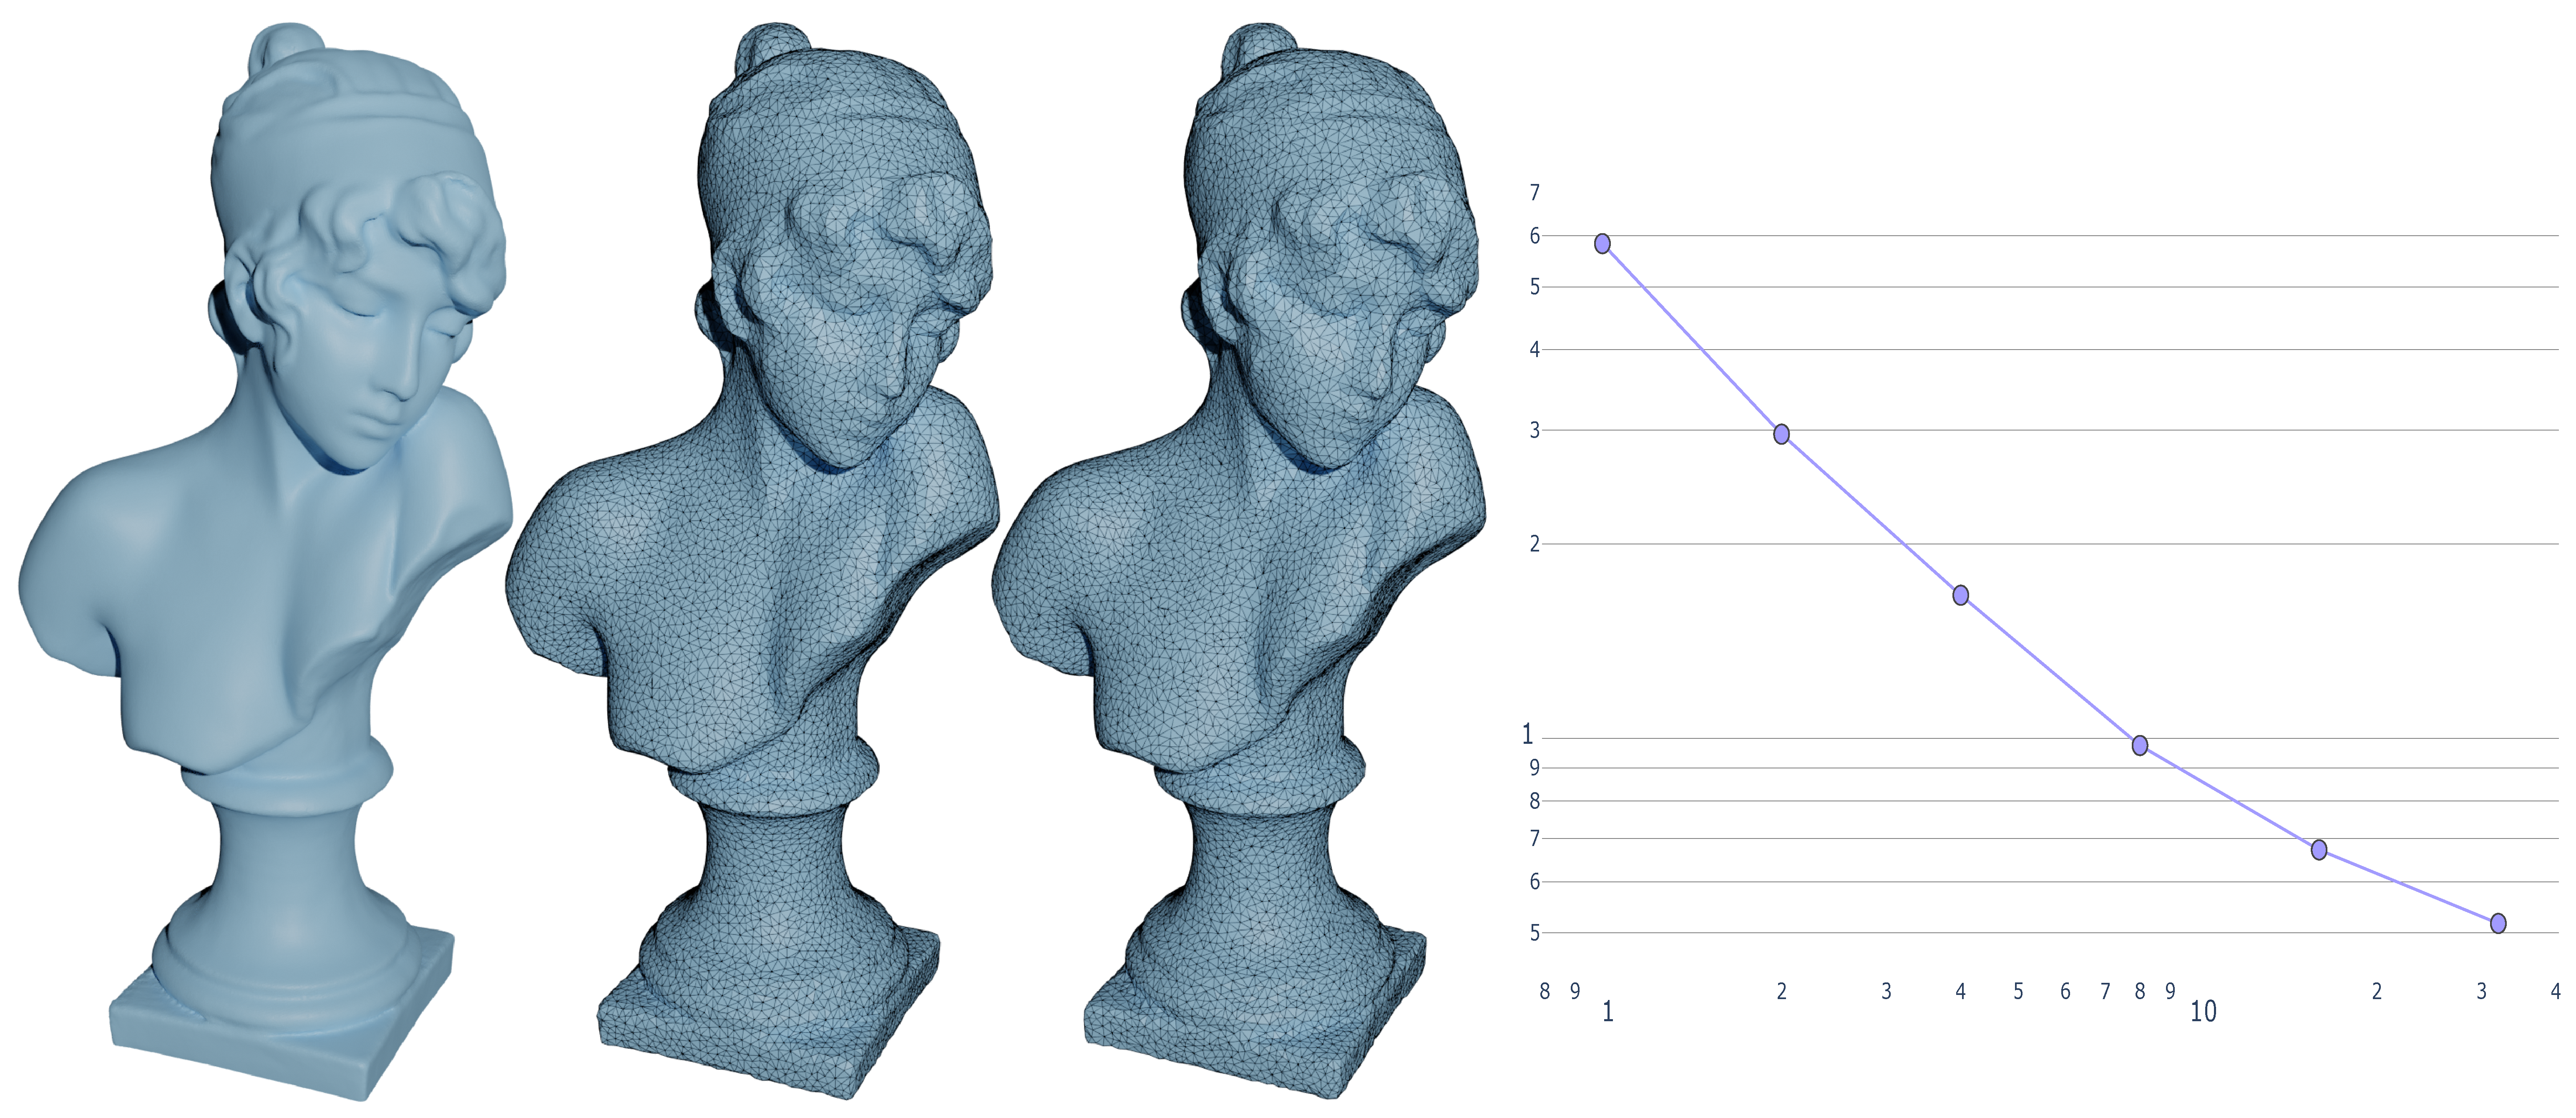
\includegraphics[width=\linewidth]{wmtk-tex/figs/2d-sec-statue.pdf}
    \parbox{.15\linewidth}{\centering Input}\hfill
    \parbox{.15\linewidth}{\centering libigl}
    \hfill
    \parbox{.15\linewidth}{\centering Output}\hfill
    \parbox{.3\linewidth}{\centering Timing}\par
    \caption{
    Comparison of our parallel implementation (32 threads) of shortest edge collapse (scalability plot on the right, from 1 to 32 threads) of a model with $281,724$ faces with the serial version in libigl. {Both libigl and our output have $28,168$ faces and comparable edge length (1.058 for libigl versus 1.061 for ours). Our serial method runs in 4.9s (5.84s on a single thread, 0.52s with 32 thread, leading to a speedup of $11\times$), while libigl runs in 2.74s.}}
    
    % 0 thread: 4.9s
    % 1 thread: 5.84s
    % 2 thread: 2.96s
    % 4 thread: 1.67s
    % 8 thread: 0.98s
    % 16 thread: 0.67s
    % 32 thread: 0.52s
    \label{fig:decimate}
\end{figure}

\paragraph{QSlim}
{We use our framework to implement QSlim~\cite{garland1997surface}. 
QSlim collapse edges based on the planarity of the two adjacent faces measured with an error quadric. The algorithm continues to collapse until it reaches a target number of edges. We compare our implementation with the QSlim implementation in libigl \cite{jacobson2016libigl}. The serial libigl implementation is 8 times faster than our implementation, due to their direct manipulations of elements in the queue with each collapse. But our parallel implementation is twice as fast when using 16 threads (Figure \ref{fig:qslim})}.

\begin{figure}
    \centering\footnotesize
    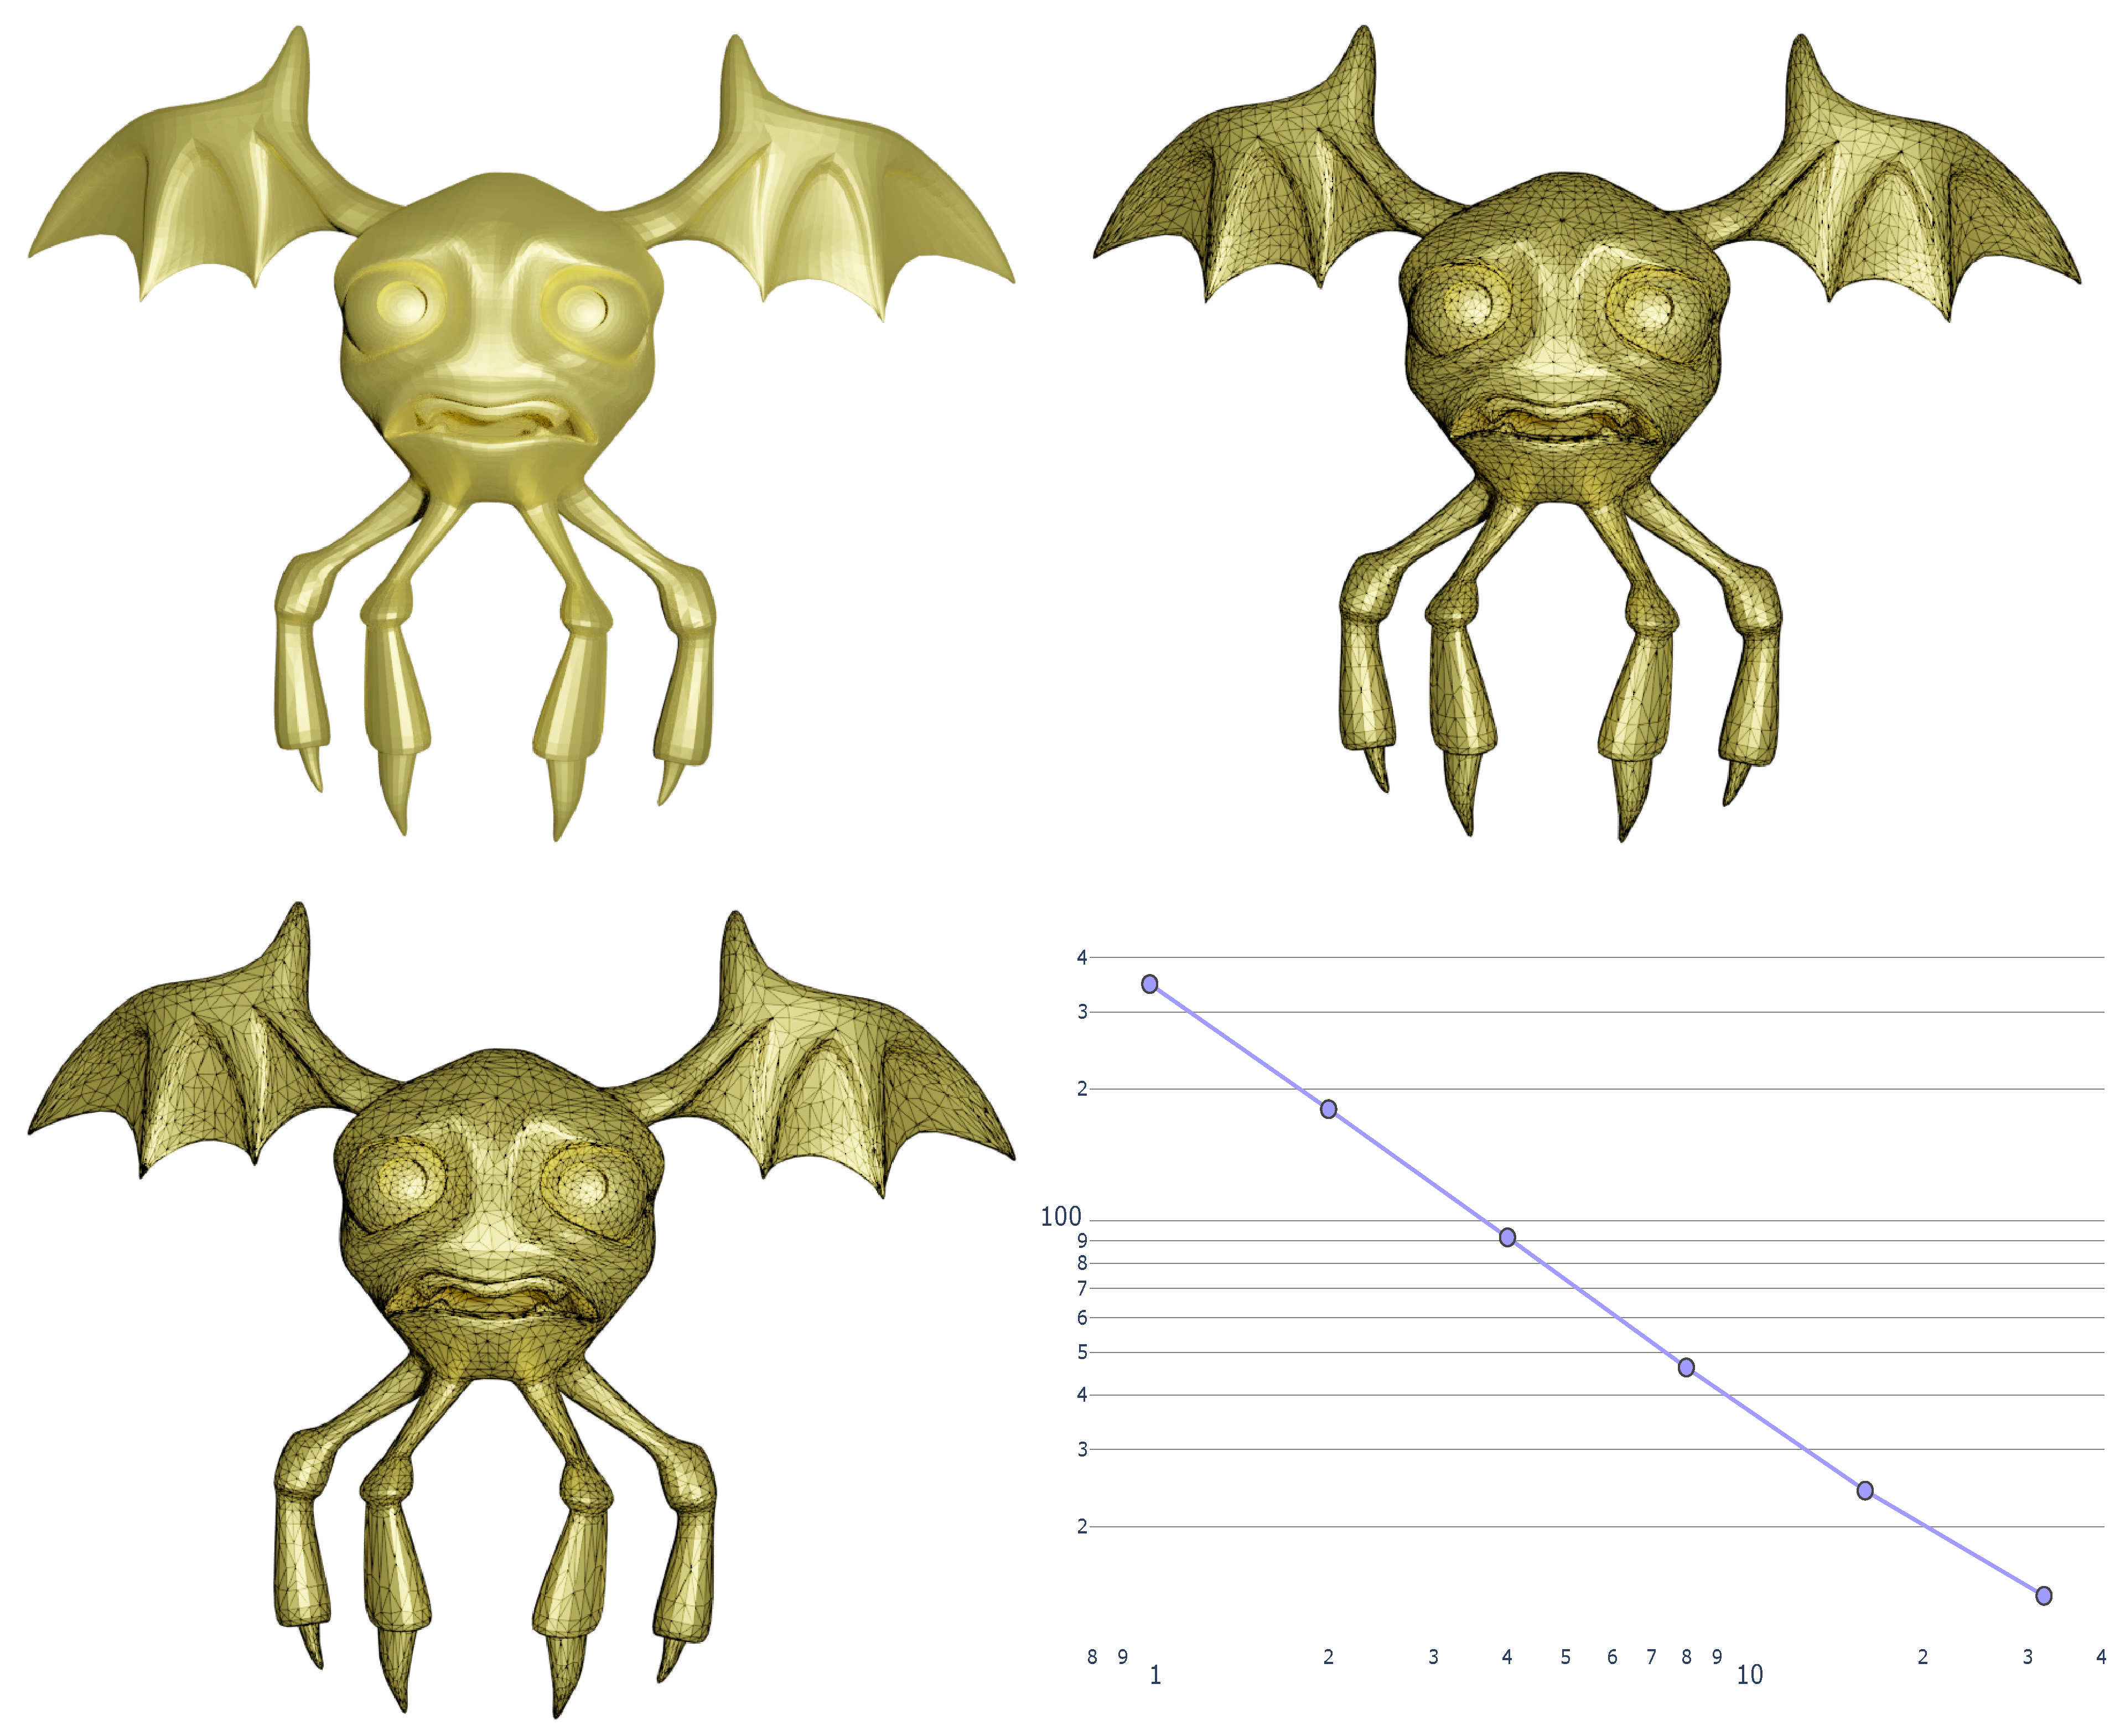
\includegraphics[width=\linewidth]{wmtk-tex/figs/2d-qslim.pdf}
    \caption{{Comparison of our parallel implementation of QSlim with the serial version in libigl for a model with $1,909,755$ faces. Top right, the libigl output has $17,891$ faces and takes 41.26s. Bottom left, our output has $17,906$ faces and runs in 306.59s.  Our implementation scales well: 347.59s with one thread and 13.88s with 32 (25$\times$ speedup).}
    }
    \label{fig:qslim}
\end{figure}

    % 0 thread: 306.59s
    % 1 thread: 347.59s
    % 2 thread: 179.84s
    % 4 thread: 91.62s
    % 8 thread: 46.19s
    % 16 thread: 24.16s
    % 32 thread: 13.88s

\paragraph{Isotropic Remeshing}

We implemented the {widely used} algorithm for isotropic remeshing proposed in \cite{botsch2004remeshing}. This algorithm alternates edge collapse, edge flips, edge splits, and tangential smoothing to obtain a mesh that is isotropic (i.e. all elements have the same size) and where all triangles are close to equilateral. The process is guided by a user-provided target edge length $L$, and terminates when no local operation leads to either an improvement in the desired edge lengths or an improvement in vertex valence \cite{botsch2004remeshing}.

In Figure~\ref{fig:uniform}, we compare our implementation of \cite{botsch2004remeshing} with the implementation in OpenFlipper~\cite{mobius2010openflipper}.
The OpenFlipper implementation is 2.5 times faster when running on a single thread, and our implementation becomes faster after 4 threads are used (Figure \ref{fig:uniform}).

\begin{figure}
    \centering\footnotesize
    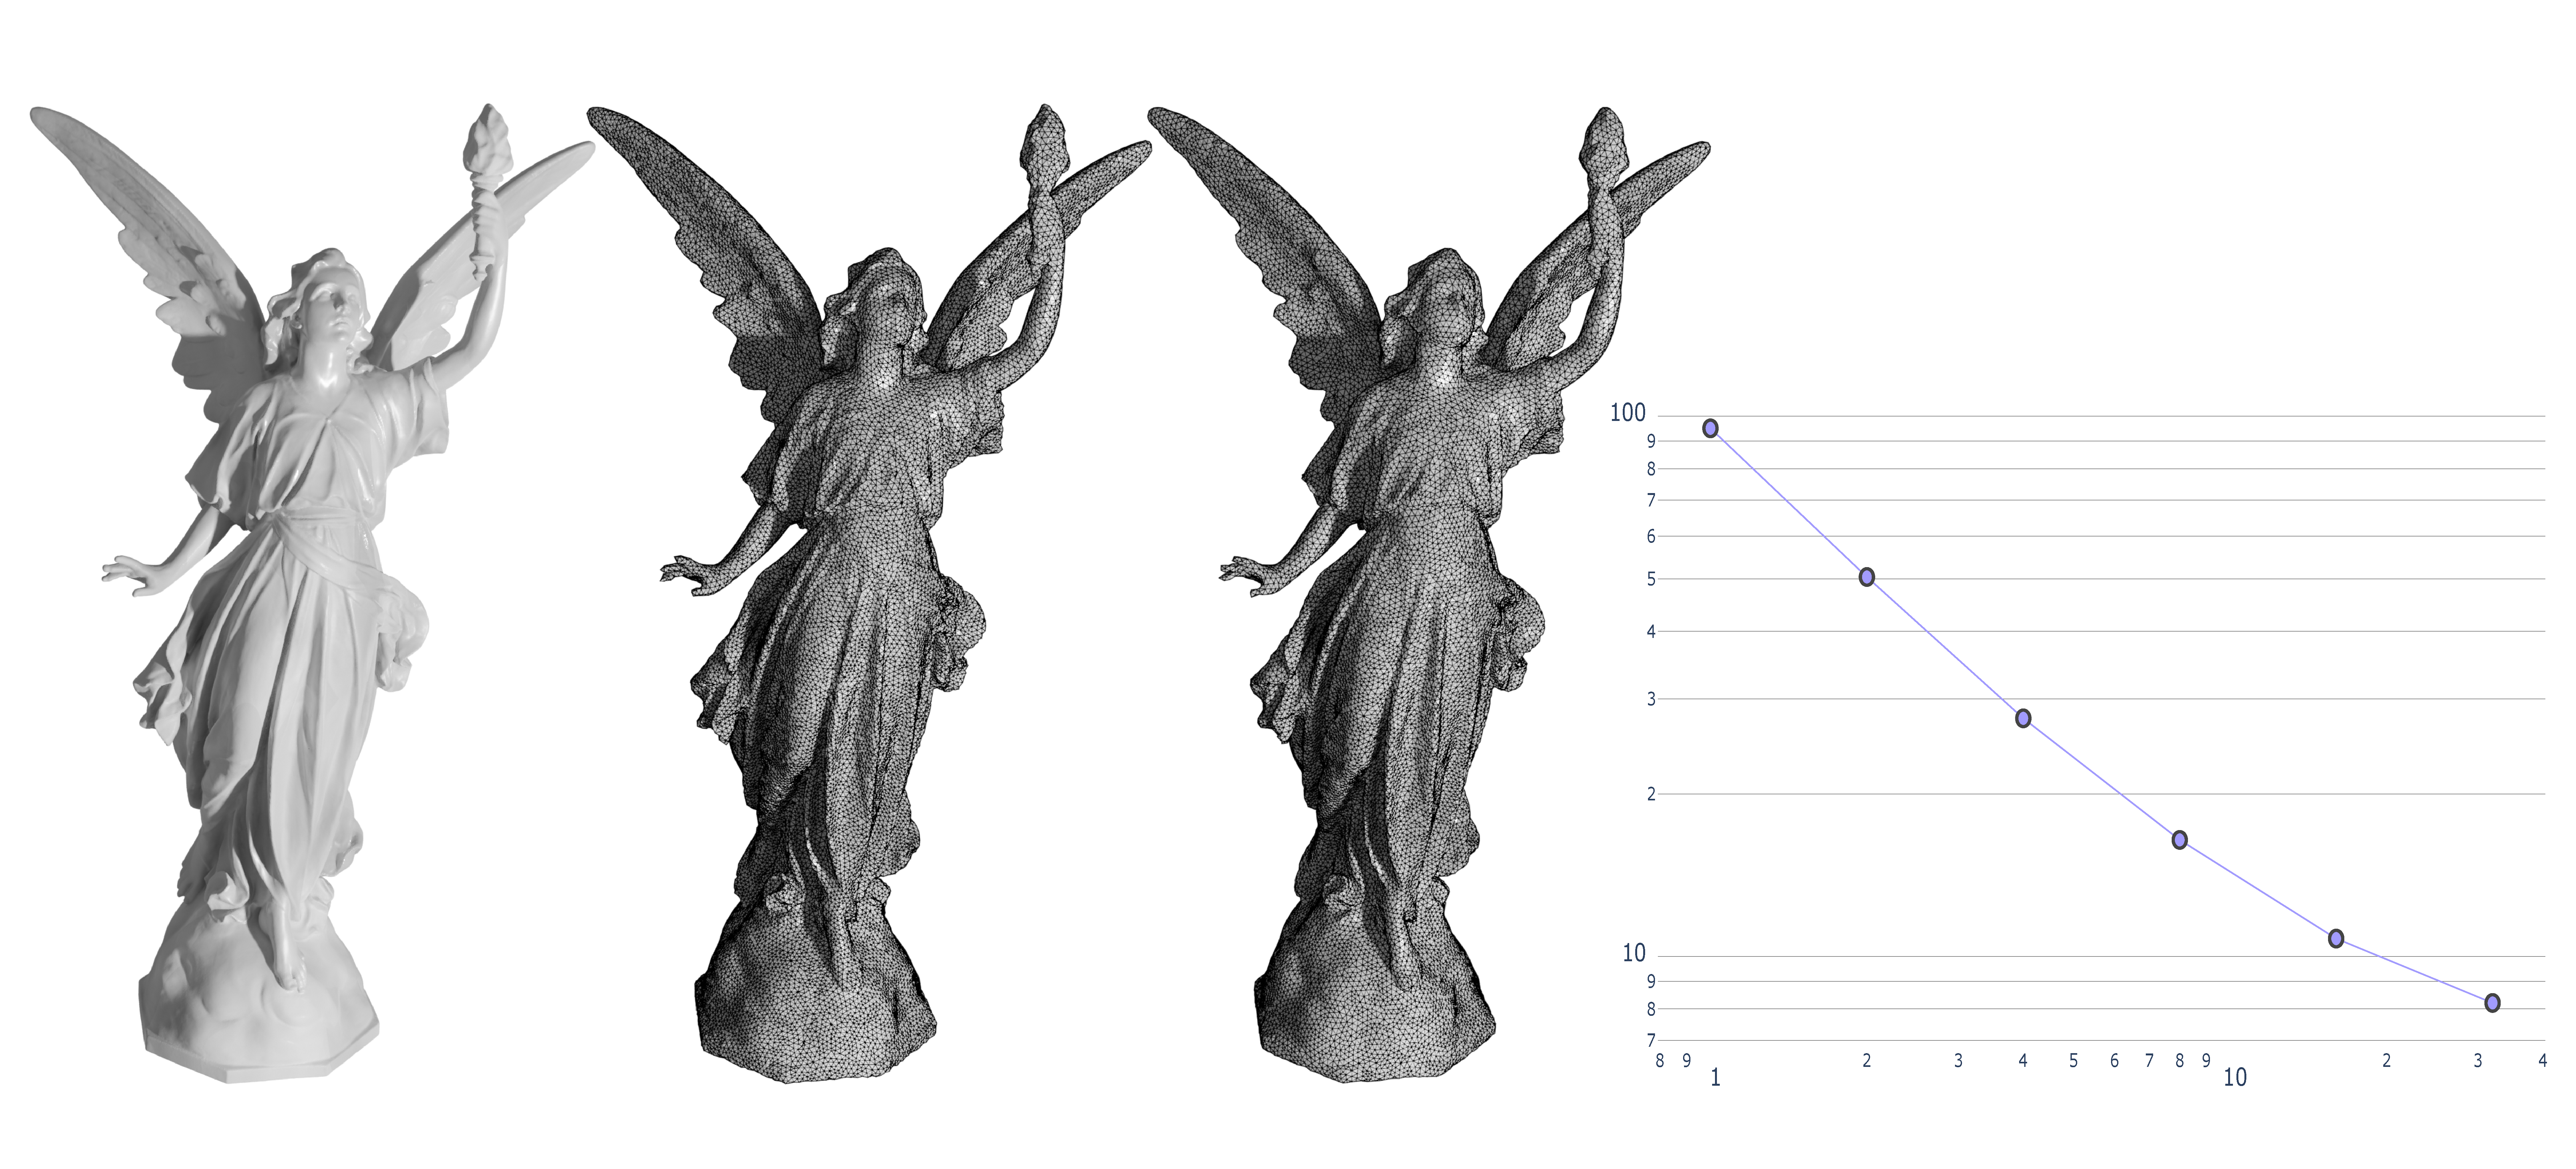
\includegraphics[width=\linewidth]{wmtk-tex/figs/2d-remeshing-lucy.pdf}
    \caption{Example of uniform remeshing a model with $2,529,744$ triangles (left) with the same target edge length. Middle, \cite{mobius2010openflipper} remeshes it to $78,322$ faces in 31.96 seconds. On the right is our
    32-thread implementation, which generates $71,640$ triangles in 8.2 seconds (78.34s serial, 95.0s for a single thread, leading to a speedup of 11$\times$). The difference in density of the meshes is due to differences in the detail of the implementation, which makes the two methods reach an average vertex valence of 5.999, and a similar target edge length (differ 0.01\% of the bounding box diagonal length) with a different element budget.}
    \label{fig:uniform}
    % wmtk avg length 8.86, opf: 8.59, BB 1922.46
    % openfliiper 31.96s
    
    % 0 thread: 78.34s
    % 1 thread: 95.0s
    % 2 thread: 50.42s
    % 4 thread: 27.6s
    % 8 thread: 16.44s
    % 16 thread: 10.8s
    % 32 thread: 8.2s
    
\end{figure}

\paragraph{Harmonic Triangulations}

The \emph{harmonic triangulations} algorithm has been introduced as an alternative to sliver exudation in the Delaunay tetrahedralization pipeline to efficiently reduce sliver tetrahedra. The original paper \cite{Alexa:2019} proposes to use both flip and smoothing operations. 

The code provided by the authors implements a reduced version of the algorithm proposed in the paper, restricting the optimization to 3-2 edge swap operations. We thus implemented both a reduced version for a fair comparison (Figure \ref{fig:harmonic}) and a complete version. Our more generic framework is twice as slower than the hand-optimized code written by the authors when running serially, and it is 2 times faster when running on 32 threads (Figure \ref{fig:harmonic}).

% Reference: 
% Total time for harmonizing Delaunay triangulation: 6.37256 seconds
\begin{figure}
    \centering\footnotesize
    \includegraphics[width=\linewidth]{wmtk-tex/figs/3d-harmonic-gauss.pdf}
    % \parbox{.2\linewidth}{\centering Input\\\#V = 1 million}\hfill
    \parbox{.2\linewidth}{\centering Reference}\hfill
    % \\\#T =6MM,  6.37 s\\Mean Harmonic Index 0.547}\hfill % 5.25 on Kirby, 6.38 on sonic
    \parbox{.2\linewidth}{\centering Output}\hfill
    % \\\#T = 6MM, 3.82 s (32 threads) \\Mean Harmonic Index 0.554}\hfill
    \parbox{.3\linewidth}{\centering Timing}\par
    \caption{Example of \emph{Harmonic Triangulations} starting with one million Gaussian distributed random points. {Both our and the reference implementation reach a similar target number of tetrahedra (5.9 million for the reference and 6.1 million for ours, due to a difference in operation ordering) and a similar Mean Harmonic Index (0.547 for the reference and 0.554 for ours). Our method takes 3.82s with 32 threads (15.49s serial, 40.49s on a single thread, speedup of 11$\times$), while the reference serial implementation takes 6.37s.}}
    \label{fig:harmonic}
    
    % harmonic: 
    
    % 0 thread: 15.49s
    % 1 thread: 40.49s
    % 2 thread: 21.6s
    % 4 thread: 12.3s
    % 8 thread: 7.27s
    % 16 thread: 4.99s
    % 32 thread: 3.82s
    
\end{figure}

\paragraph{Tetrahedral Meshing}

The TetWild algorithm is a tetrahedral meshing algorithm with minimal input requirements: given an input triangle soup, it can generate a tetrahedral mesh which approximates its volume. We {take inspiration from} the original algorithm introduced in \cite{hu2018tetrahedral,Hu:2019:fTetWild} with a few modifications: (1) we use the insertion operation \cite{Hu:2019:fTetWild} (using rational coordinates) as a replacement for their BSP partitioning, as this simplifies the implementation, (2) we use the envelope proposed in \cite{Wang:2020:FE} instead of sampling, and (3) we use 2-3 face swapping, 3-2 and 4-4 edge swapping operations, to simplify the implementation. We show results on two models in Figure \ref{fig:tetwild}: the results are very similar to the original implementation, and our version is 2 times faster when using 8 threads. {We experimentally observe that our framework scales well up to 8 threads, after that the algorithm becomes slower. This is because, as we increase the number of threads and partitions, the frequent conflict in tetrahedral mesh edge operations affects the parallel performance. We believe that this observation might be useful for the future design of high performance concurrent mesh generation algorithms.}
% faster now!
% latest.  original: 287.577s


% 0 thread: 452.42s
    % 1 thread: 521.47s
    % 2 thread: 300.48s
    % 4 thread: 197.68s
    % 8 thread: 153.33s
    % 16 thread: 176.82s
    % 32 thread: 207.35s
% 0.000000000000000000e+00,4.524295280000000048e+02
% 1.000000000000000000e+00,5.214727839999999333e+02
% 2.000000000000000000e+00,3.004886300000000006e+02
% 4.000000000000000000e+00,1.976867799999999988e+02
% 8.000000000000000000e+00,1.533386629999999968e+02
% 1.600000000000000000e+01,1.768291299999999922e+02
% 3.200000000000000000e+01,2.207351280000000031e+02


\begin{figure}
    \centering\footnotesize
    \includegraphics[width=\linewidth]{wmtk-tex/figs/3d-tetwild-dragon.pdf}
    \caption{Tetrahedralize a surface with $856,294$ faces. Original TetWild (top right) generates a mesh with $56,761$ tetrahedra in 287.58s; our reimplementation (bottom left) generates a mesh with $44,866$ tetrahedra in 153.33s with 8 threads (452.42s serial, 521.47s on a single thread, speedup of $3.4\times$). The difference in number of tetrahedra is likely due to the different order of scheduling of operations due to the partitioning.}
    \label{fig:tetwild}
\end{figure}

\subsection{Parallelization}
{
Enabling the parallelization mechanism introduces a minor slowdown as visible in the difference between the pure serial and one thread timings on our applications, due to the additional cost of allocating mutexes and to acquired them. The algorithm scales well in all 5 applications (figures \ref{fig:decimate}, \ref{fig:qslim}, \ref{fig:uniform}, \ref{fig:harmonic}, \ref{fig:tetwild}), obtaining a scaling speedup. 
%Our speedup is 11 \DP{check, 11 in both?} in triangular mesh applications with 32 threads and 11 \DP{11 gain?} in tetrahedral mesh applications using 32 threads. 
We would like to remark that thanks to our specification and our runtime, the serial and parallel implementation of the 5 algorithms above is almost identical.}

{An inevitable drawback of parallelization is that the algorithms cannot efficiently preserve ordering. For instance, in shortest edge collapse, every thread will try collapse edges in its own partition independently from the others. If one of these collapses append on the partition's interface, the thread will need to acquire a lock. In case of failure the collapse is postponed to a later stage thus not respecting the order (Figure~\ref{fig:limitation}). This is a rare event that is more problematic for fast operations.}


\begin{figure}\centering\footnotesize
    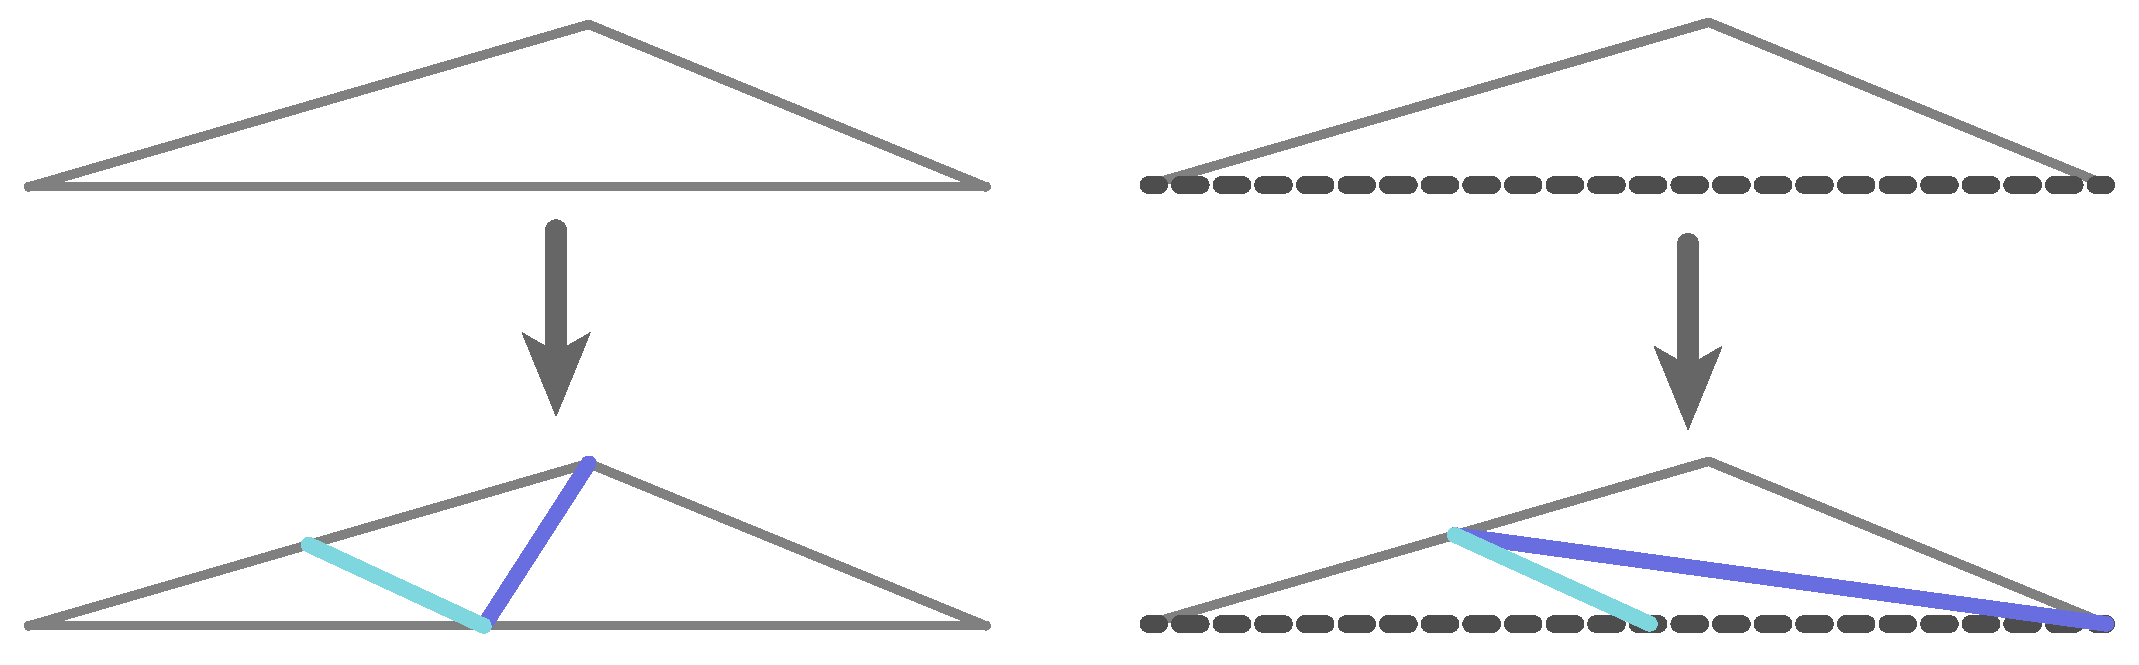
\includegraphics[width=\linewidth]{wmtk-tex/figs/limitation-of-para.pdf}
    \caption{{Example of splitting the longest edge on the bottom of the triangle. On the left, the edge can be split to generate the dark blue edge. In the next iteration, the left edge is split (by the light blue edge) leading to a decreasing maximum edge-length. On the left, the bottom edge is locked illustrated by a dashed line. In this case the next iteration splits the left edge (dark blue edge) and so on. As long as the dashed edge is locked it will never be split preventing the maximum edge length to decrease.}}
    \label{fig:limitation}
\end{figure}

\subsection{Algorithm Modifications}

A major motivation to invent and develop this declarative language is enabling easy customization of meshing algorithms. As an example, we add an additional termination criteria to the shortest edge collapse and uniform surface refinement.  Integrating the envelope check is straightforward with our approach, as it only requires adding the envelope check to the invariants. We use the open-source library proposed in \cite{Wang:2020:FE}, which allows to directly specify the maximal allowed surface deviation. The envelope adds a noticeable computational cost, which is ameliorated by our parallel implementation (figures \ref{fig:decimate_envelope} and \ref{fig:uniform_envelope}). 

\begin{figure}
    \centering\footnotesize
    \includegraphics[width=\linewidth]{wmtk-tex/figs/2d-sec-envelope.pdf}
    \parbox{.3\linewidth}{\centering Input}\hfill
    \parbox{.3\linewidth}{\centering Output}\hfill
    \parbox{.3\linewidth}{\centering Timing}\par
    \caption{Shortest edge collapse with envelope containment of a model with $857,976$ faces. {Our method successfully generates a mesh with $71,298$ faces in 37.49s with 32 threads (731.32s serial, 725.34s on a single thread, speedup of $20\times$).}}
    \label{fig:decimate_envelope}
    
    % 0 thread: 731.32s
    % 1 thread: 725.34s
    % 2 thread: 397.18s
    % 4 thread: 220.58s
    % 8 thread: 117.26s
    % 16 thread: 63.55s
    % 32 thread: 37.49s
    
\end{figure}


\begin{figure}
    \centering\footnotesize
    \includegraphics[width=\linewidth]{wmtk-tex/figs/2d-remeshing-headport-env.pdf}
    \parbox{.3\linewidth}{\centering Input}\hfill
    \parbox{.3\linewidth}{\centering Output}\hfill
    \parbox{.3\linewidth}{\centering Timing}\par
    \caption{Uniform remeshing with envelope containment check of a model with $198,918$ faces. {Our method produces a mesh with $68,202$ faces in 29.11s with 32 threads and 493.54s for a single thread (483.68s for the serial version) leading to a speedup of 16$\times$.}}
    \label{fig:uniform_envelope}
    
    % 0 thread: 483.68s
    % 1 thread: 493.54s
    % 2 thread: 258.88s
    % 4 thread: 139.36s
    % 8 thread: 77.38s
    % 16 thread: 43.16s
    % 32 thread: 29.11s

\end{figure}




\subsection{{Large-scale dataset validation}}

{To validate our framework we run our reimplementation of uniform remeshing and tetrahedral meshing on the Thingi10k dataset~\cite{zhou2016thingi10k}. We run all experiments serially on an individual node of an HPC cluster an Intel Xeon Platinum 8268 24C 205W 2.9GHz Processors limiting the runtime to 15 hours.}

{For uniform remeshing,  Figure~\ref{fig:2d-datasaet} shows the time, average edge length normalized by the target, and average valence of isotropic remeshing on the ten thousand models. Most of our models finish within 10 seconds with only a few requiring more than a minute. For almost all meshes, the algorithm succeeds at reaching the target edge length and valence of 6.}

{For TetWild we limit the number of iterations to 25 (Figure~\ref{fig:3d-datasaet}). 
We note that within the 15 hours limit only 2.5\% models did not finish, and after 25 iterations 3\% of the models still have some rational coordinates. Among the successful models, most finish within 20 minutes and succeed in achieving high-quality meshes (only 8 models have average AMIPS larger than 10). 
}


\begin{figure}
    \centering\footnotesize
    \includegraphics[width=\linewidth]{wmtk-tex/figs/tri2d-stats.pdf}
    \caption{{Timings, target edge length ratio, and valence for every model in the dataset. Most models finish within a minute. The target edge length ratio measure how well our algorithm simplifies the meshes to reach the desired edge length, with an optimal value of 1. Since uniform remeshing strives to generate regular meshes, for most model our algorithm is able to obtain the optimal valence of 6.}}
    \label{fig:2d-datasaet}
\end{figure}


\begin{figure}
    \centering\footnotesize
    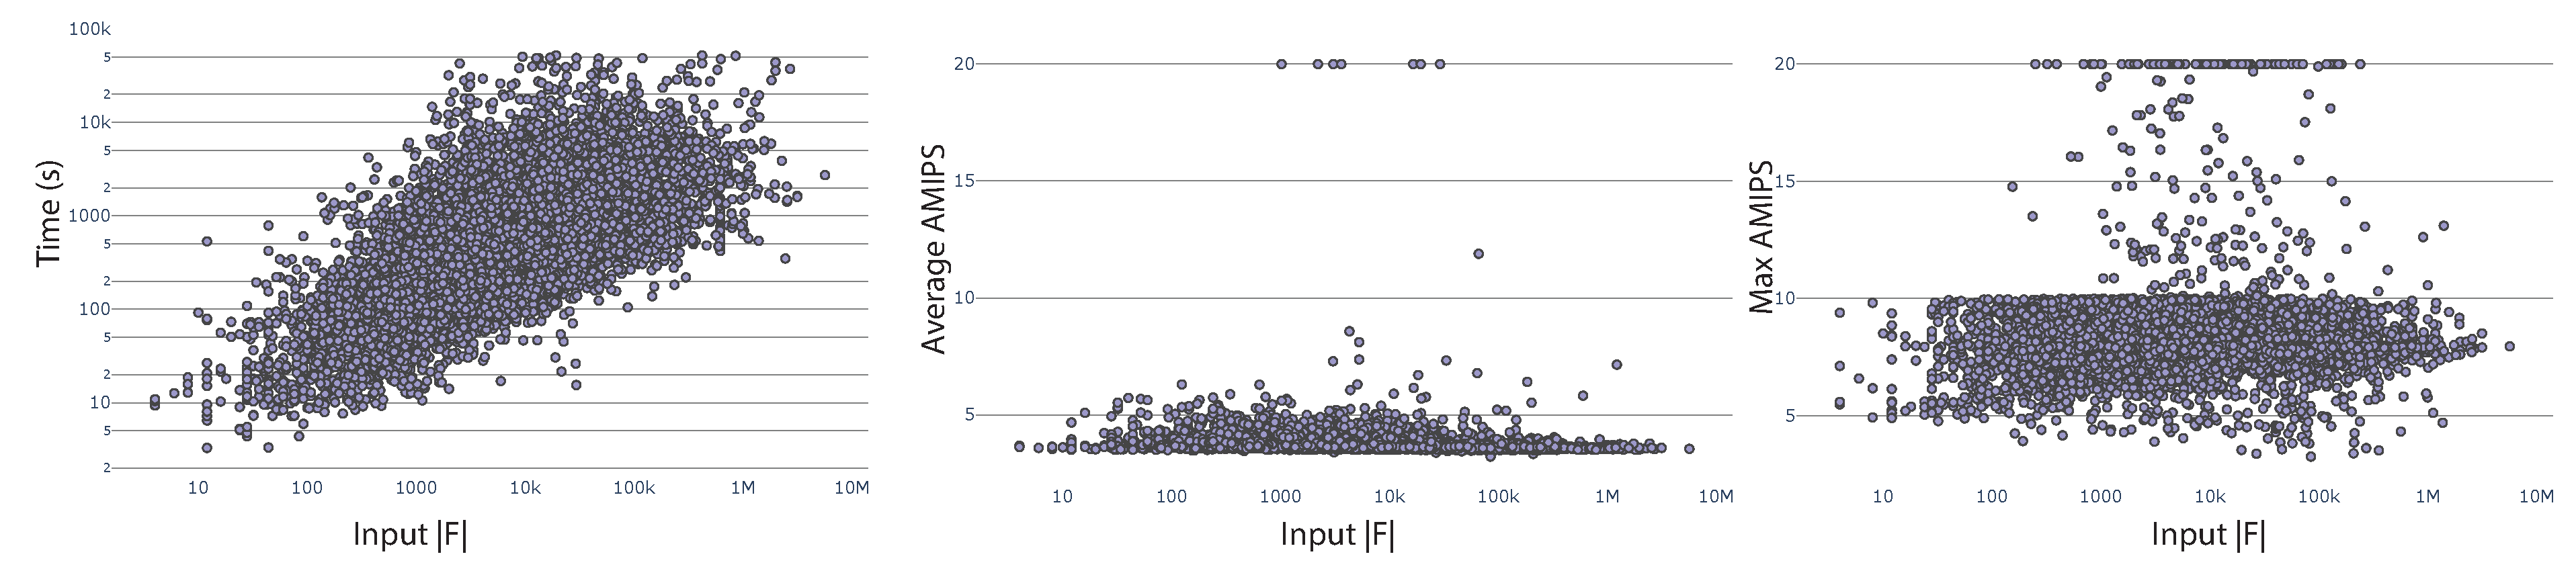
\includegraphics[width=\linewidth]{wmtk-tex/figs/tet3d-stats.pdf}
    \caption{{Timing, max and average AMIPS energy (capped at 20) for maximum 25 iterations of tetrahedral meshing. Most models finish withing 20 minutes with only a few taking up to a day. Even by limiting the iterations to 25, most models reach an average AMIPS energy lower than 10, with optimal value at 3.}}
    \label{fig:3d-datasaet}
\end{figure}
